\chapter{Requirements}

The conclusion of the game engine analysis laid the foundation for forming the requirements presented in this chapter...
% Skriv dette men bedre :)

Based on the game engine analysis, we made some requirements which is stated in this chapter

\todo{Conclude the game engine analysis - you}

The client stated their initial requirements in the form of one main goal and two sub-goals. The main goal was to create a demo which satisfied their requirements. They also presented two sub-goals, to an in-game model placing tool, and an in-game railway builder. Our requirement document are based on these requirements, but does also extends further. This chapter goes over the specific requirements set for the project by the client, the group itself, and the industry standards.


\section{Functional Requirements}

To display and visualize the core functionalities of our simulator we have chosen to utilize use cases. Use cases provides a structure and overview of the functionality works as a tool to force awareness for the requirements in the development phase. 

There was a quite unanticipated issue with defining use cases for the project as an entirety. Our main goal is, as stated previously to make a demo in the chosen engine and also make the code applicable for further development. What we discovered in the development of the demo was that the classes and structures we created often laid a groundwork for further development. We therefore decided to include two separate groups of use cases for our project. One for the application it self, and one for the use cases that got facilitated by us through development. The reasoning for including this is for the client to more easily understand the functionality and it requires us to focus on the code quality and further development perspective of the project.

\todo{sammenheng mellom use cases og issues}

\subsection{Use Case Diagram: Application}
The use case diagram illustrates all available actions for the two groups of users; students and employees. While not implied in the diagram to avoid cluttering, it should be noted that an employee has access to all functionality of the student.
\begin{figure}[H]
\centerline{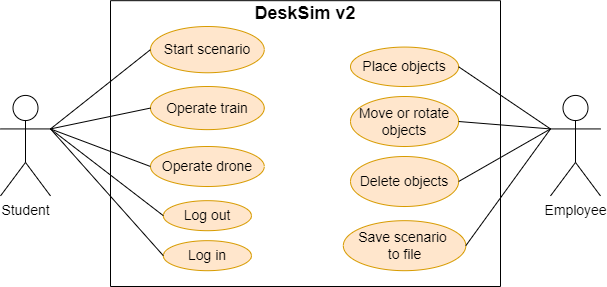
\includegraphics[width=1.0\textwidth]{figures/Desksim usecase-Final.drawio.png}}
\caption{Application use case diagram}
\label{use_case_engine}
\end{figure} 

\textbf{High Level Use Case}
% PLACE OBJECTS
\begin{table}[H]
    \centering
    \begin{tblr}{colspec={|X[.2, l]|X[.8, l]|}, hlines}
        \textbf{Use Case:} & Place objects \\
        \textbf{Actors:} & Employee \\
        \textbf{Goal:} & To place the necessary objects such as a train and a railway in a level. \\
        \textbf{Description:} & When a level is opened in editor mode the user is provided a user interface which includes a content browser. The user can click on a item in the content browser and drag it out in the level. The content browser has different categories the user can select in the top bar by clicking on the category buttons.
    \end{tblr}
    \caption{Use Case: Place objects}
\end{table}
% DELETE OBJECTS

\begin{table}[H]
    \centering
    \begin{tblr}{colspec={|X[.2, l]|X[.8, l]|}, hlines}
        \textbf{Use Case:} & Delete objects \\
        \textbf{Actors:} & Employee \\
        \textbf{Goal:} & To delete an object in the level. \\
        \textbf{Description:} & When clicking on an object in a level the user will be given the option to remove it. After the click, the user will get a trash can symbol at the top bar, next to the transformation options. After clicking on the trash can, the program will prompt the user for confirmation before permanently removing the object from the scene.
    \end{tblr}
    \caption{Use Case: Delete objects}
\end{table}

% OPERATE DRONE
\begin{table}[H]
    \centering
    \begin{tblr}{colspec={|X[.2, l]|X[.8, l]|}, hlines}
        \textbf{Use Case:} & Operate drone \\
        \textbf{Actors:} & Student \\
        \textbf{Goal:} & Maneuver the drone camera \\
        \textbf{Description:} & The student switches to drone view. This lets them move around freely in all three dimensions, forwards/backwards, horizontally, and vertically. The user can also use the mouse to freely look around in the world, and adjust the movement speed of the camera.
    \end{tblr}
    \caption{Use Case: Move or rotate objects}
\end{table}

\textbf{Low Level Use Case}

% NEW, move or rotate object
\begin{table}[H]
    \centering
    \begin{tblr}{colspec={|X[.2, l]|X[.8, l]|}, hlines}
        \textbf{Use Case:} & Move or rotate objects \\
        \textbf{Actors:} & Employee \\
        \textbf{Goal:} & To move a object or rotate it into the prosition and position you want \\
        \textbf{Precondition:} & The user has successfully opened a scenario in editor-mode \\
        \textbf{Success Scenario:} & 
        
        \todo{Skriv om - Thomas}
        
            1. The employee selects an object by clicking on it. \newline
            2. The object displays a gizmo, either in the form of arrows for moving it along each of the three-dimensional axes, or a wheel to rotate the object. \newline
            3. The user changes the mode to the one he want from the top bar icons. \newline
            
            4. \textbf{For translation:}\newline
                5. The user hovers the mouse over the arrow to select one axis, or in the middle of two arrows to select a plane. \newline
                6. The user drags the mouse to the position he wants the object to be located \newline
                
            4. \textbf{For rotation:} \newline
               5. The user presses the wheel and drags the mouse around the wheel to get the desired rotation. 
    \end{tblr}
    \caption{Use Case: Move or rotate object}
\end{table}


\begin{table}[H]
    \centering
    \begin{tblr}{colspec={|X[.2, l]|X[.8, l]|}, hlines}
        \textbf{Use Case:} & Operate Train \\
        \textbf{Actors:} & Student \\
        \textbf{Goal:} & To drive the train in a scenario \\
        \textbf{Precondition:} & The user has successfully opened a level and the levers is connected to the system through a USB port \\
        \textbf{Success Scenario:} & 
            The user accelerates or decelerates the train using the levers or the keyboard \newline
            %1. The user pushes the left lever or the keyboard to accelerate the train. \newline
            %2. The user pushes the right lever or the keyboard to apply break force on the train. \newline
            Depending on the scenario, the user has to follow some rules: \newline


                The user should not exceed the speed limit. Doing so should result in system regulated brakes turned on. \newline
                
                The user is provided information about the current speed in the Driver Machine Interface. \newline
                
                The user should follow the rules regulated by signals: \newline


                    \textbf{Main signal:} If this signal is red the user should stop. If user don't stop before the signal this should result in breaks turned on.
                    
                    \textbf{Main signal:} One green light means that the user can drive with reduced speed.
                    
                    \textbf{Main signal:} Two green lights means that the user can and should continue with the set speed.

    \end{tblr}
    \caption{Use Case: Operate Train}
\end{table}

\section{Use Case Diagram - Game engine}


\begin{figure}[H]
\centerline{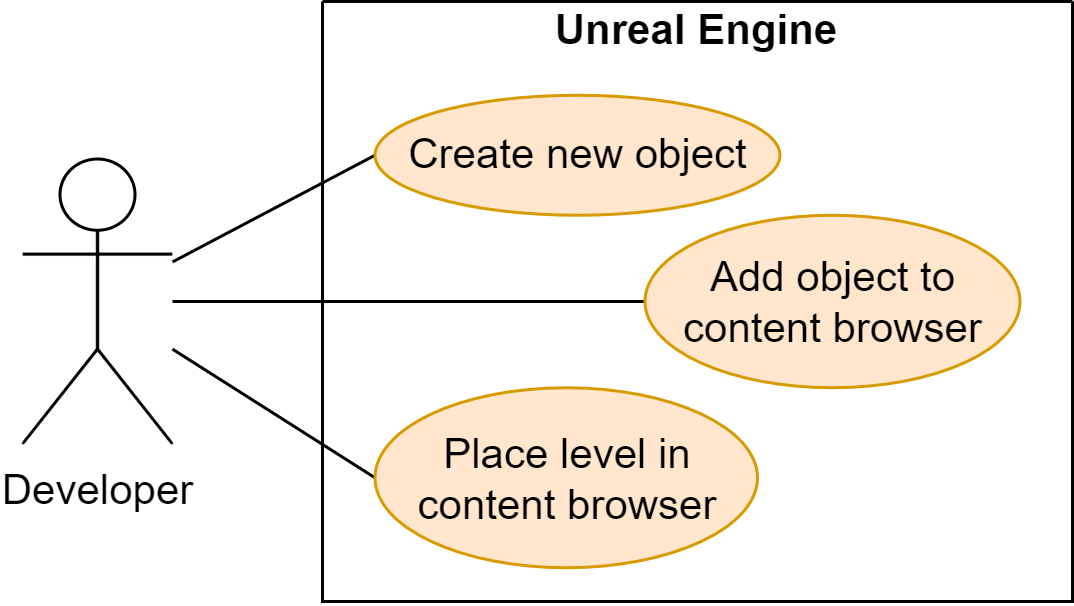
\includegraphics[width=0.9\textwidth]{figures/UEUseCase.png}}
\caption{Game Engine use case diagram}
\label{use_case_application}
\end{figure} 

\textbf{High Level Use Case}
\todo{fjern spesifikke steps og unreal objects}
\begin{table}[H]
    \centering
    \begin{tblr}{colspec={|X[.2, l]|X[.8, l]|}, hlines}
        \textbf{Use Case:} & Add Level in Main Menu \\
        \textbf{Actors:} & Developer \\
        \textbf{Goal:} & To add a level created in unreal engine to the simulator. \\
        \textbf{Description:} & When the developer has created a scene he wants to be a part of the simulator he must know the name of the level. The level name is stored as a FName, and the content browser only need its value. The FName's are immutable and case sensitive so it's important to have the right name. Open the MMObjects inside \textit{BP\_EditorHUD} blueprint located in "\textit{DeskSimV2/Source/DeskSimV2/Editor/UI}". The developer now clicks the + button to add the new level and fills in the name, description and the FName reference to the map. 
    \end{tblr}
    \caption{Use Case: Add Level in Main Menu}
\end{table}


\textbf{Low Level Use Case}


\todo{Change them from intructions to use case description}
\begin{table}[H]
    \centering
    \begin{tblr}{colspec={|X[.20, l]|X[.75, l]|}, hlines}
        \textbf{Use Case:} & Add new object \\
        \textbf{Actors:} & Developer \\
        \textbf{Goal:} & To add a new object to the game \\
        \textbf{Preconditions:} & The developer has a working version of Unreal Engine version 4.27.2 or higher. The developer has a 3D model he wants to be added in the game.  \\
        \textbf{Success Scenario:} & 

            1. The developer adds a new model to the "models" folder inside Unreal Engine \newline
            2. The developer registers the new object by deriving a new blueprint from the \cpp class relevant to the objects category.\newline
            3. The developer selects the new model as the blueprint's static mesh.\newline
            4. The blueprint is compiled and saved.\newline
            %2. The developer navigates to "C++ classes" in the content browser. \newline
            %3. The developer right clicks on either "BasicStaticObject", "Train" or "BasicSignal" or "wagon", based on what item type the object is.\newline
            %4. The developer clicks on "Derive blueprint from c++ class..." in the drop-down menu and selects the appropriate place to store the blueprint.\newline
            %5. The developer opens the blueprint and drags the imported model from step 1 into the "Static mesh" variable in the details panel for the object.\newline
            %6. The developer compiles and saves the blueprint \newline
    \end{tblr}
    \caption{Use Case: Add new object}
\end{table}
\todo{Change them from intructions to use case description}

\begin{table}[H]
    \centering
    \begin{tblr}{colspec={|X[.20, l]|X[.75, l]|}, hlines}
        \textbf{Use Case:} & Add object in Content Browser \\
        \textbf{Actors:} & Developer \\
        \textbf{Goal:} & To successfully add a created object in the content browser making it clickable and draggable in runtime.\\
        \textbf{Preconditions:} & The developer has created a new object as described in the "Add new object" use case.  \\
        \textbf{Success Scenario:} & 
        
            1. The developer opens the blueprint for the Editor-HUD.\newline
            2. The developer adds a new item to be registered as an object.\newline
            3. The developer fills in the category, name and description for the object.\newline
            4. The developer adds a reference to the actor asset.\newline
            
            It is required to close out of the application and regenerate the project files or rebuild the solution with visual studio before the object shows up in the content browser.
            %1. The developer open the \textit{BP\_EditorHUD} blueprint located in "\textit{DeskSimV2/Source/DeskSimV2/Editor/UI}". \newline
            %2. The developer clicks on the \texttt{+} icon for the CBFObjects. \newline
            %3. The developer adds the category the actor should be a part of.\newline
            %4. The developer writes a suitable name and description for the object. \newline
            %5. The developer adds the reference to the actor he wants to include.\newline
            
            %6. Close unreal engine desktop and visual studios and navigate to the file system for the project. Right-click on the \textit{DeskSimV2.uproject} files and select "generate visual studios project files" from the dropdown menu.\newline
            %7. The item should be visible and draggable in-game in the content browser. \\
        
        %\textbf{Alternative Scenario:} & 
        
            %6. Open visual studio and right click on DeskSimV2, select "rebuild" and let the solution rebuild. \newline
            %7. When its built, open DeskSimV2.uproject and check if the object is added.
    \end{tblr}
    \caption{Use Case: Add object in Content Browser}
\end{table}


\subsection{Operational Requirements}
These are the requirements which concerns the application at it's operational stage, this stage begins at the project's deadline which is the 20th of May:
\begin{itemize}
    \item The application must be able to interact with the existing Rest-API hosted by Lokførerskolen.
    \item The system must operate on Windows devices.
    \item The system must manage privileges of users and only allow elevated users to access the editor functionality.
    \item Must be transferable through a zip file
    \item The system must operate on computers which has 8GB of ram and a Intel® Core™ i5-4460 CPU or better. 
    \item Should not experience frame rate drops of lower than 60 frames per second. 
\end{itemize} 


\subsection{Security and Misuse}
\label{OperationalRequirements}
To ensure the security of the users and avoid misuse of the application the application:
\begin{itemize}
    \item must require user authentication for usage. The authentication process should be a token based system where you receive a token. The token has an expiration and should be used to authenticate the user up to its expiration. When the token expires the user will be asked to authenticate again and receive a new token. % er dette operational?
    \item should not contain bugs and/or security flaws that potentially could lead to harm or destruction of hardware components. Such flaws include bad memory handling.
    \item must not store any passwords in plain text.
\end{itemize}


\subsection{Interface Requirements}
\textbf{Menus} 
\begin{itemize}
    \item It should  be intuitive and easy for a student at Lokførerskolen to navigate the Main Menu. 
    \item The Main Menu should have the same functionality as the previous simulator and only deviate by design.
    \item All text must be available in Norwegian.
    \item Buttons should be intuitive to reduce the number of operations required for a task.
\end{itemize}

\textbf{Scenarios} 
\begin{itemize}
    \item The game should have an option to switch between a Drone Mode and a Train Mode. 
    \item The \acrshort{dmi}  viewport in a game should be responsive to the gameplay and be movable for the player.
    \item All numbers and measurements must be specified in the metric system.
\end{itemize}